\chapter{Afterword}

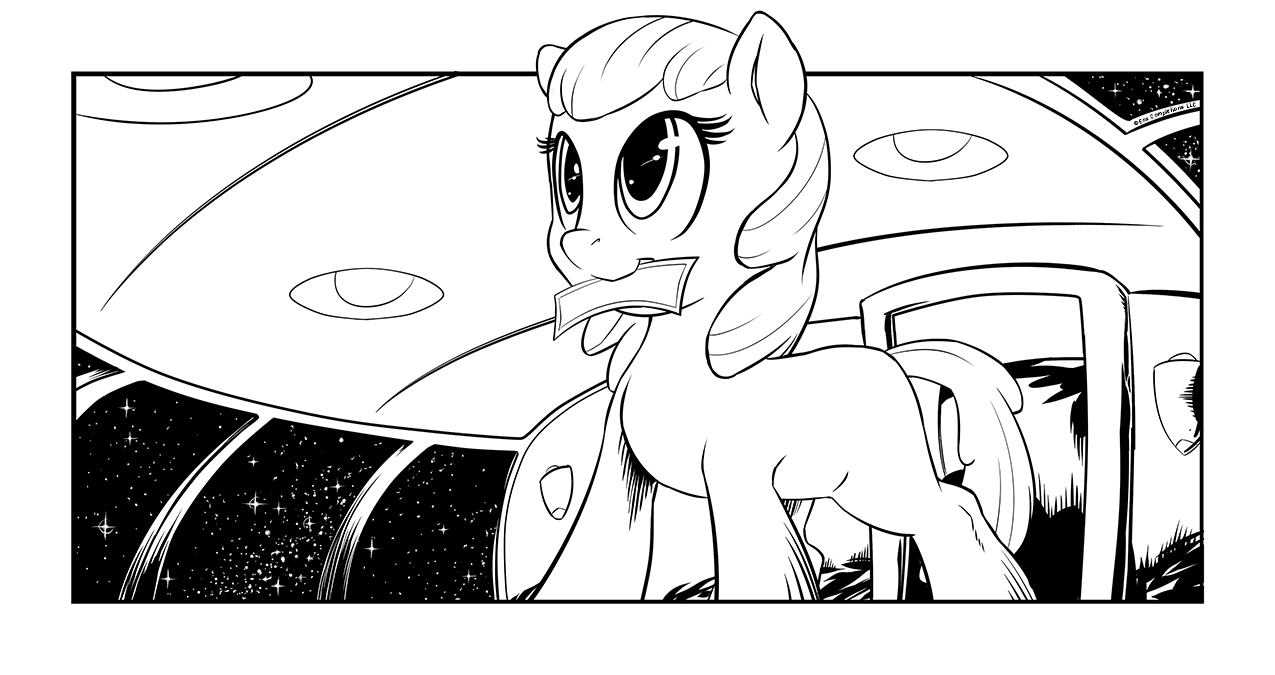
\includegraphics[width=\linewidth]{image21.png}

\begin{intro}
    Beyond the horizon, we will be together again.
\end{intro}

{\rt

``Oh, c'mon, you can't st- FZZT -rking right now!'' BAM BAM BAM! ``Hello hello? Test, test\dots onetwothree\dots''

``\dots''

``Okay, it seems to work. Very well\dots let's get started. First of all, my name is Watcher. My self imposed mission was to watch over the Wasteland, looking for lost ponies and groups of adventurers, hoping to eventually find those that carried the Elements of Harmony. Now, things are changing and I have friends that will help me with my task. I'm not alone anymore, and I finally have some time for doing things that I feel need to be done.

``And this is the reason why now I'm recording this tape and, just for this tale, I'm asking you to call me Mister Questioner. This is a story that could seem unimportant, or even silly, but it's about dreams, and memories. It's a story about two large, innocent pink eyes that couldn't see the horrors of our times and kept believing that somewhere, behind those ruined walls, inside the slave pens and even in the raiders' camps, everypony was still a pretty pony.

``And at the end of her journey, where the road met the ocean, the ghost foal that lost her mom finally found a place to rest. Sure, she was a little late, but I was told that when she finally accepted her fate, Puppy left with a smile.

``Like she were following an old postcard the filly went down the Big 52, showing everyone she met what ponies had been in the past and what they could still be. Somehow changing the way they saw themselves, making them see a better past, and making them wish for a better tomorrow. She wasn't actually trying to change the world, or even to save lives, but that might have been why so many ponies took notice. Since she was no preacher but simply herself, it was easy to see that there was no fanaticism or weird ideals in her; just a little pony with large pink eyes that knew, for a fact, that no one could really be that evil.

``And this\dots this is what happened in the few months between Puppy's arrival at Emerald Shores and today.

``The ponies of Emerald Shores came back to the town shortly after the Wild Herd's defeat: when they arrived from the NCA, they found the graves on the hill and the remains of the crushed ferris wheel; alas, what really startled them was that somepony had changed the name of the town on all the signs. Now the town is called Nightmare's Fall.

``The survivors of Ironworks started rebuilding the town, helped by their neighbours. Since the battle the settlement had a shortage of adult ponies, so the Rangers decided to settle in this town, making it their new headquarters. Not everypony was happy with this new situation, but the rangers proved themselves vital during the liberation of the town, and eventually even the most stubborn came to accept them.

``With Ivory Tower destroyed and Ironworks reduced at the shadow of its former self, Broccoli gathered all the ponies that didn't want to live in a ghost town or hadn't a home in which to live at all. The work in the fields improved greatly and the farmers diversified their crops, for the joy of the foals. Now they grow both broccoli and cabbage.

``The crater at Ivory Tower was filled by the seasonal rains and a small trading post has been built along the route between Broccoli and Rust Manor. The town is very small and lightly fortified, but it's growing fast and somepony is starting to build farms all around the lake. The town still doesn't have a name, but the traders call it The Hole.

``Rust Manor was attacked during the Enclave conflict; the town wasn't able to repel the attackers and the control tower was completely destroyed; numerous ponies were killed, but the survivors are already beginning to rebuild their home. It won't be easy, but nothing is easy in the wasteland.

``Sun City is still a war zone. The Sand Sweepers and a number of small bands are currently fighting each other to gain the control of the desert's gem. Since the Hired Hooves retreated from Sun City during the Enclave conflict and never came back, the settlement is still a dangerous place, avoided by almost every caravan. For those that dare to risk their lives, though, the inner town is full of old world technology that could make you rich for the rest of your life.

``Tunnel Town expanded on both sides of Sugartop Mountain and now it's the third largest town along the Big 52. The prices for using the tunnel have been cut considerably and the city began a service of long range patrols to keep at bay the groups of raiders and slavers along the Route in the town's territory.

``Salt Cube City is still the biggest city along the Big 52 and it has grown even more since the ghouls left the Dome. The Hired Hooves are expanding their influence even outside the Route, and have opened offices in the nearby towns. The Talons don't seem very happy with this policy, and tension between the two mercenary groups is rapidly growing.

``The Redtrotters didn't change very much: they stayed faithful to their tribal customs and are still charging the caravans that travel along their territory, but now foals don't have to pay the fee. This is not a big improvement, but the tribe has opened relations with the other settlements and they are actually trying to improve the safety of their part of the Route.

``The Applejack Rangers helped in reconstructing Ironworks, establishing their new base in the town's Stable. During the last battle at the Cave, all four of Ironworks' surviving paladins were dispatched to help with defending the place, and I had the opportunity to meet both Cold Shower and Scold. The battle was hard and Shower didn't survive it; she is now sleeping besides Gauss at Emerald Shores. Scold has grown distant after losing her; it seems that the old scribe is doomed to survive all his friends\dots a fate that I can easily understand.

``Happy and Jamie married and I was told that she is expecting. Since the marriage is quite a recent news, I think that they didn't expect to be celebrating again so soon. When asked what name they are planning to give the foal, Happy stated that she's still uncertain, but it won't be Puppysmiles.

``Molten Gold didn't stop his graverobbing career for long after the battle with the Nightmare. The ghoul left as soon as he recovered and sailed south on a steamboat, along with a group of adventurers. I haven't heard anything from him since then.

``SolOS and Pinkie 7 were actually able to become friends in the end. I was contacted by P7 a little after the first Enclave attacks; she was curious about this 'Questioner' Puppy was always talking about, so we had a chat and even if I don't think I'm going to trust her or SolOS any time soon, I think that they aren't going to give us troubles for a while. She actually scared me a bit when she told me about her and SolOS' idea of programming a new AI and naming it Puppy.SML\dots I hope that this was just a joke.

``Lonesome Pony recovered from his wounds and went back to Radio 52, keeping the Big 52 together with his encouraging speeches and all of his music. DJ Good Stuff is still working with him but when I tried asking when they were going to marry, both of them laughed at me. During the Enclave conflict Radio 52 kept broadcasting; it was small enough that the pegasi didn't bother to shut it down. The radio helped with organizing the defenses and boosted the morale of the defenders; it wasn't very much, but it was enough for those that fought during the conflict.

``Mister White trotted back to Salt Cube City; the loss of Sage Brush changed him deep inside, even if his sister never blamed him for it. After resigning his place of leadership, he became a traveling merchant and as far as I know, he's still running along the Route, bartering every sort of merchandise. This is just a rumor, but it seems that one of his guards is a unicorn mare with a tower as a cutie mark. Maybe he didn't want to lose the opportunity to hire somepony that had the guts to spank a Nightmare, or he simply wanted to give a raider a second chance\dots After all you gotta care, right?

``After Long Ears' demise, a new filly in her tribe got the Far Seer cutie mark, becoming the next shaman. I have no idea how their power works, but it seems to be some mix of powerful drugs and innate precognition; I just know that it is very tolling and quickly consumes the mare's body, so that a single pony sacrifices her life to help the tribe. A boon that brings a curse\dots

``There's still a pony that I never met in person, and I'm starting to doubt his actual existence. Puppy described him to me as\dots the baddest evil villain ever. Count Horse Tile. I asked several travelers and caravan guards, but no one has been able to give me a single clue about this cruel noble pony\dots I guess his mystery will remain unsolved.

``Henrietta is still running from the Talons. It seems that there has never been good blood between them and the Firebrights, and the young griffon is keeping up the family tradition. I tried to talk with Gawdyna, to see if some sort of truce can be arranged. I hope that Henry will accept to parley; after all she was Puppy's best friend, and seeing the girl die because of a feud that she didn't even start is something i rally don't want to see.

``The Wild Herd was dispersed and fled to their outposts on the coast again. This time they suffered heavy losses, both in numbers and in pride, but everyone knows that they will come back one day. Hopefully, even if they once more strike the Big 52, it will be without the help of an army of robots, and that could be enough to let the good ponies sleep quietly, for the moment.

``The Lost Herd seems to be gone. With Sidekick's death, the last of those damned souls found peace at last, and finally Equestria will be able to forget one of the many horrors of the war. May those poor foals find a deserved rest in whatever awaits us past this life.

``So, this is the end of Puppy's story. Did she really change something along her path? Will her action matter in the long run? I have--- sorry, I \emph{has} no idea, but I think I'll miss the way she talked, and the way she took everything so lightly. Another shard of the Equestria I loved is forever gone\dots but I still hope that I will live long enough to be able to see a filly like her again; but this time it won't be a ghost from the past, but a daughter of the present.

``And speaking of ghosts, the legend of the Ghost of the Big 52 is still alive, even if it seems more a Nightmare Night's tale than a real story. It's said that when the sun goes down and the moon is waning, a ghostly figure rides along the Route, silent like a shadow and swift like the wind. It looks for the souls of the wicked: slavers, raiders and the evildoers that lurk in darkness, waiting for easy prey. At least two groups of raiders were actually found dead along the route: they didn't show a single wound, their weapons were still fully loaded and they were clearly ready to strike\dots but they died on the spot, with no explanation. Killed by a presence that didn't leave a single clue. So, now I want to ask you one thing.

``Do you believe in ghosts?''

}

\horizonline

\englishdaytimeplace{4}{7:30 P.M.}{Downtown, Salt Cube City}

Sand Box turned the wheel left trying to make the airship fly against the wind, but it was an impossible task. Friend Force One was losing pieces along the way since the take off, and two engines had already failed. The ghoul slammed his hoof down on the intercom and yelled: ``Soft Air, we need more power! We're getting pushed back by a damn nightly breeze! I don't know how, but give me more knots!''

The reply from the communication device had more in common with an electrocution than an actual conversation, but it was about the balloon losing gas and the engines catching fire.

Sand box cursed, before talking again in the instrument. ``Okay don't worry, I've got a backup plan: we will crash the airship here, so that the wind won't send us back to Salt Cube city!''

If the reply from the other side of the line was a complaint, it never reached Sand Box. In that very same moment the whole world decided to become pure light.

Just an endless, blinding, perfectly silent light that enveloped everything. There was no pain, and there was no fear. Just light.

\horizonline

\englishunknowndaytimeplace

When Sand Box opened his eyes again he had the unsettling feeling that there was absolutely nothing wrong. Nothing at all. He took his time to look for a moment around the flying deck, trying to understand what happened. Well, the wheel was still there, the sky was all starry, the commands were working, the lights were all lit\dots

``Wait a moment\dots the lights are all lit? There are stars outside? What the\dots''

Yes, the airship was working perfectly, and by perfectly it meant that the whole damn room seemed as new as the day it went out from the docks. The floor was shining, the commands were clean, the wheel was even waxed! And the windows! They were so clear that you could even see yourself inside th---

And Sand Box saw Sand Box. Surprise on his muzzle was giving way to realization. Slowly, he touched his face with a hoof. It was\dots his real face, the one he had before becoming a ghoul! He was a pony again, he was\dots

Dead.

He was dead, this was the only possible reason for all of this. But if he was dead, why was he still on the ship? Was this some sort of afterlife punishment where he had to fly a ship forever, like the Flying Dutchmare? Were the others trapped forever on that thing with him? And why? He\dots he didn't want to fly forever, he had to see Agatha! She\dots she was waiting for him somewhere, he couldn't just\dots fly a stupid ship for the eternity!

FWEEEEET! A loud whistle interrupted Sand Box's shipwreck of desperation, making him turn towards the deck's entrance. A feminine voice announced her arrival while the door slammed open. ``Captain on the Bridge!''

A pink mare with a pink mane and big blue eyes appeared in front of the former ghoul; she was wearing a navy officer uniform and sported the largest smile Sand Box had ever seen on a pony\dots ``Miss\dots Minister Pie?''

Pinkie dismissed Sand Box with the wave of a hoof. ``Ah, call me Captain Pinkie, I don't like that ministry thing\dots it wasn't happy at all anyway.'' The young mare started jumping in every corner of the bridge, giggling and yelling enthusiastically. ``Yay! I knew that this little filly was going to fly sooner or later! Oh, oh, look! Look at this! All the arrows on the panels are pink exactly as I asked! It's\dots it's fantastic!''

The chief technician stood still with a confused expression on his muzzle, looking at the hyperactive pony touching everything while moving around at a speed that wasn't physically possible. ``I\dots can I help you somehow?''

Before Sand had the time to finish the question, he found himself staring into Pinkie's enormous blue eyes, nose to nose with her. ``Sure you can! They are all waiting for you in the lounge! Move that slow rump of yours and join the party! I'll get there as soon as I'm done having fun here!''

The stallion nodded, slowly stepping back towards the door and never losing eye contact with Pinkie Pie. She was a little bit scary, especially from the point of view of a pony that had just been dead for less than ten minutes. Once on the stairs, he turned on his tail and rushed to the airship's recreational bridge.

The saloon wasn't crowded, still it was quite populated, especially since Sand Box clearly recalled that aboard the Friend Force One there were just four ponies when it took off. Now instead he counted eight guests.

It was easy to recognize Soft Air from his typical military technician jumpsuit, and Peach Blossom with her blooming peach flower cutie mark was easy to spot; the middle aged mare with the stethoscope had to be Dr. Get Well\dots wow, she was quite a sight with all of her skin and muscles in their place\dots This left a griffon and four other ponies that Sand Box didn't recognize.

The griffon was sipping tea while reading a newspaper, sitting on a couch. He was wearing combat armor and had several weapons on him. Two of the ponies, a mare and a stallion, had the typical padded suit used under power armor and were standing side by side in front of a table with drinks and snacks. They didn't pay attention to the table anyway, being too occupied in nuzzling each other, seemingly at peace.

The third pony was sitting alone in front of a window, looking outside the ship. He sighed and shook his head, in his eyes was easy to read some sort of regret and resignation. As if he left too many things undone behind and wanted to go back. The fourth pony was a unicorn mare with a long cape; she had the Sand Sweepers traditional jewelry on her, maybe she was a dead far seer? The mare seemed different from the others, more a shadow than a real presence. She was also the one that trotted towards Sand Box when he stepped inside the room.

``Greetings, I see that Pinkie let you come down at last. I guess this means that we are ready to proceed\dots she should be here soon, unless she got lost again.''

Sand Box frowned. ``What is going on? Who is she? Who are you? Listen, I'm not a troublemaker but I'd---'' He stopped talking when the mare approached a door and pulled it open. A Pink foal with a blond mane and two big pink eyes trotted inside the room.

Puppy still had her pretty silver ticket in her teeth. She didn't understand how exactly she arrived in that place, but it didn't matter. There were games, and treats, and it totally seemed like a super fancy party! It was everything she always dreamed, and it was full of ponies to boot! And a Chicken!

Sand Box felt his heart sink in an icy grasp. Of all the ponies he was expecting to see, Puppysmiles was the last one. ``Oh, little one\dots I'm\dots I'm so sorry\dots'' How could this foal smile even in a moment like this? ``What happened? Who\dots how did you arrive here?''

Puppy tilted her head, unable to recognize the pony in front of her, but he seemed very nice, so it was all right. ``Hi mistur pretty pony! I am Puppysmiles, and I am going to find my mom! A super nice skelly pony gave me this super fancy ticket and sent me here! And I was told that Mom was just over there, after the ride!'' The little filly paused for a moment, checking the place. ``Ah, are we there yet?''

Sand Box blinked his eyes, trying to understand what the foal meant, but Long Ears came in his help, whispering in his ear, ``Her mother is dead\dots'' This only succeeded in making Sand's perplexity grow.

``You\dots you are happy to be dead?''

Puppy giggled. ``The nice skelly pony told me so, mistur pretty pony! But I feel fine and I'm going to find mom! This is, like, the best thing ever!''

``B-but\dots'' She was so\dots happy\dots and even if she was explained what was going on, what would have been the point of it? Sand Box smiled and nodded. ``Yes. Yes it is. Do you want to play something with the others until we arrive?''

In the meantime, the various ponies in the room had slowly gathered around Puppy. They were all looking at her with various degrees of perplexity or sadness. Cold Shower and Gauss approached the filly, the mare was the first to talk.

``I'm sorry that we had to fight you\dots I wish there was a better way\dots'' Gauss nodded for a moment, sighing deeply.

``Ah, why is everypony sad? Where are the pony games? I want to play hide and seek! Or pin the tail on the pony! And then I wanna dance, and\dots Oh, I hope the pony tail is pink! Pink is my super favorite color! I'm the bestest tail pinner ever!'' Puppy was already jumping on her hooves, trying to look beyond the small group of ponies.

Pinkie, now wearing a flight attendants uniform, followed Puppy through the door, and patted the foal on the head. ``I'm sorry Puppy, but there's no time for that! We've sailed through the Star Ocean, and now we have arrived! The ride ends here, fillies and gentlecolts! Thank you for choosing the afterlife airlines and have a pleasant stay!'' The pink mare moved rapidly towards the door, opening it and revealing to the other ponies a wonderful landscape made of green hills and small ponds.

Small herds of ponies dotted the meadows, while pegasi sat on the clouds populating a wonderful blue sky. The passengers trotted outside the ship, staring in amazement at the place. It seemed like a dream come true: here and there it was possible to see the roofs of some houses and on the distant hills there was a large apple orchard.

Even Puppy was left speechless in front of the beauty of the place; everything was perfect! The trees, the meadows, all the pretty ponies and the sunny sky! It\dots it was even better than Ponyville, it was so beautiful! The only thing that was missing was---

Puppysmiles froze for a second, her eyes staring into a small herd of ponies grazing on the borders of a daisy field. The smile on her face grew bigger and bigger as she galloped toward the ponies in the grass. One of the figures looked up and smiled at the incoming filly who was now crying with joy, unable to say anything but a single word.

``Mom!''


